
\documentclass[tikz,border=12pt]{standalone}
\usepackage{pgfplots}
\pgfplotsset{compat=1.18}
\usetikzlibrary{arrows.meta,positioning,fit,calc}
\definecolor{ink}{HTML}{172026}
\definecolor{muted}{HTML}{5F6B73}
\definecolor{line}{HTML}{CBD5E1}
\definecolor{panel}{HTML}{F8FAFC}
\definecolor{bfs}{HTML}{64748B}
\definecolor{spine}{HTML}{0F766E}
\definecolor{hrg}{HTML}{7C3AED}
\definecolor{warn}{HTML}{C2410C}
\definecolor{ok}{HTML}{15803D}
\definecolor{blue}{HTML}{2563EB}
\pgfplotsset{
  every axis/.append style={
    tick label style={font=\small, color=ink},
    label style={font=\small, color=ink},
    title style={font=\bfseries\small, color=ink},
    legend style={font=\footnotesize, draw=none, fill=none},
    grid=major,
    grid style={line!55},
    axis line style={line},
  }
}
\begin{document}

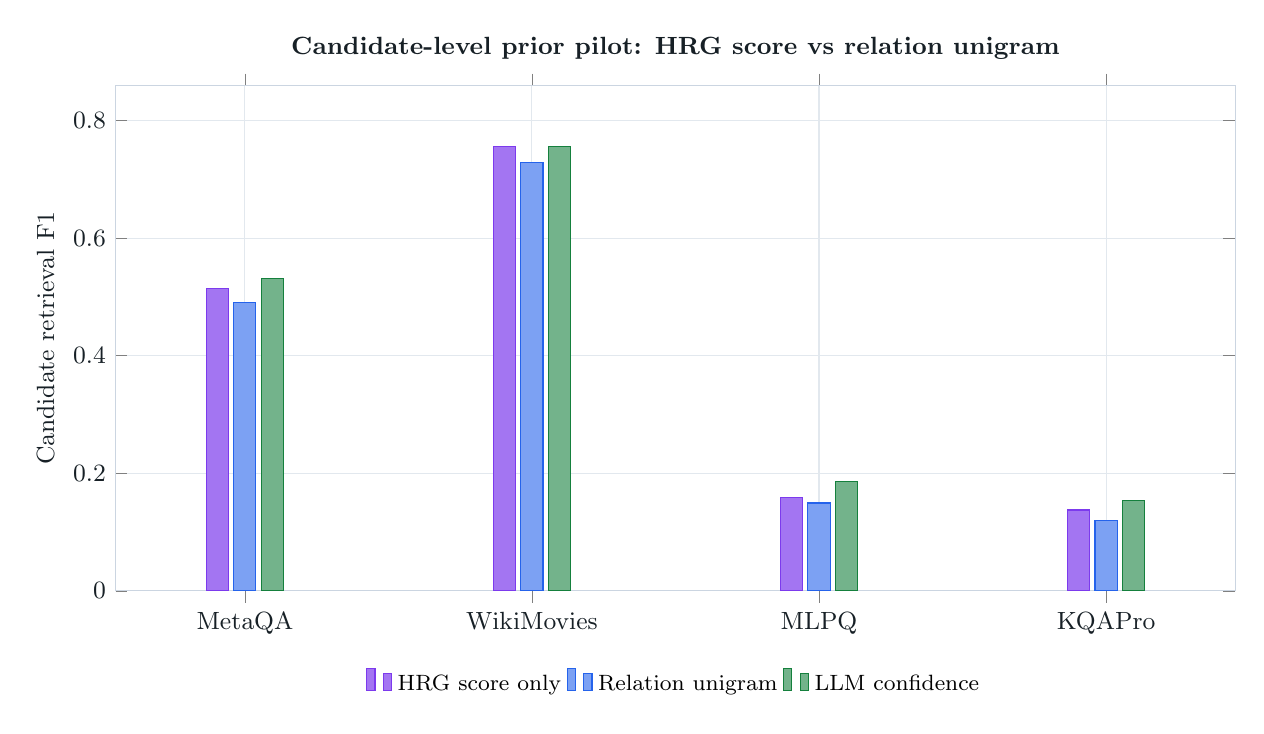
\begin{tikzpicture}
\begin{axis}[
  ybar,
  bar width=8pt,
  width=15.8cm,
  height=8.0cm,
  ymin=0,
  ymax=0.86,
  enlarge x limits=0.15,
  ylabel={Candidate retrieval F1},
  symbolic x coords={MetaQA,WikiMovies,MLPQ,KQAPro},
  xtick=data,
  legend columns=3,
  legend style={at={(0.5,-0.14)}, anchor=north, font=\footnotesize},
  title={Candidate-level prior pilot: HRG score vs relation unigram},
]
\addplot+[fill=hrg!70, draw=hrg] coordinates {(MetaQA,0.5140) (WikiMovies,0.7558) (MLPQ,0.1582) (KQAPro,0.1375)};
\addplot+[fill=blue!60, draw=blue] coordinates {(MetaQA,0.4900) (WikiMovies,0.7289) (MLPQ,0.1494) (KQAPro,0.1195)};
\addplot+[fill=ok!60, draw=ok] coordinates {(MetaQA,0.5309) (WikiMovies,0.7558) (MLPQ,0.1860) (KQAPro,0.1538)};
\legend{HRG score only, Relation unigram, LLM confidence}
\end{axis}
\end{tikzpicture}

\end{document}
